\section{Ivory's Theorem}

\begin{theorem}\label{prop:ivory}
    Consider the family of confocal conics defined by
    \[\frac{x^2}{a^2-\lambda}+\frac{y^2}{b^2-\lambda}-1=0\]
    Then the two diagonals of a  quadrangle  made of arcs of ellipses and hyperbolas have equal length. In \cref{fig:ivory} we have that $|A-C|=|B-D|.$
\end{theorem}

\begin{figure}
\begin{center}
\includegraphics[scale=0.6]{pics_08_010_ivory.pdf}
\caption{ Confocal conics and quadrangles made of arcs of ellipses and hyperbolas.}
\label{fig:ivory}
\end{center}
\end{figure}

\begin{proof} Let 
  \[ \alpha(u,v)=  \left[\sqrt {{\frac { \left( {a}^{2}-v \right)  \left( {a}^{2}-u \right) }{
{a}^{2}-{b}^{2}}}},\sqrt {-{\frac { \left( {b}^{2}-v \right)  \left( {
b}^{2}-u \right) }{{a}^{2}-{b}^{2}}}}\; \right]
\]
with $u\in [b^2,a^2]$ and $v\in (-\infty,b^2)\cup (a^2,\infty).$
\end{proof}



\section{Graves' Theorem and Periodicity}

 \begin{proposition}[{\rm\cite[{\rm  Chapitre III}]{darboux1917}}] 
 	  \label{prop:dar1} Consider two confocal ellipses $\mathcal E$ and $\mathcal{E}'$ and a point $M\in\mathcal E$. Consider the   two tangents $\ell_P$ and $\ell_Q$,  as shown in   \cref{fig:da_cordas}, intersecting $\mathcal{E}_1$ in $P$ and $Q$. Then $|MP|+|MQ|-\text{arc}{(P,Q)}=\mathrm{cte}$, where $\text{arc}(P,Q)$ is the length of the elliptic arc with extremal points   $P$ and $Q$. In particular, in a   billiard triangle $\text{conv}[P_1,P_2,P_3]$,  $|P_1P_2|+|P_2P_3|+|P_3P_1|-L(\mathcal{E}_1  )=  c_1$, where $L(\mathcal{E}_1) $ is the length of $\mathcal{E}_1$, and all the billiard triangles have the same perimeter.
 	
 \end{proposition}
 \begin{figure}
 \begin{center}
   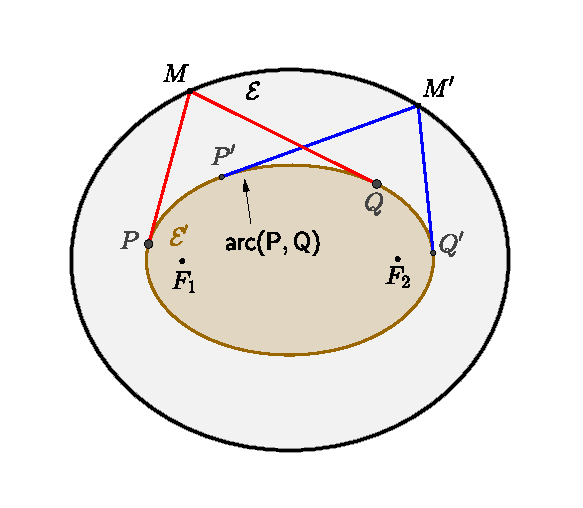
\includegraphics[scale=0.7]{pics_08_020_graves.pdf}
		\caption{ Tangents to a confocal  ellipse $\mathcal{E}'$ and invariance of the length of chords.}
		\label{fig:da_cordas}
 	\end{center}
\end{figure}
 
 \begin{proof}
 See \cite{chasles1843}, \cite[pp. 283-284]{darboux1917} and \cite[pp. 115-116]{carneiro2005}. 
 %It would be useful to obtain a proof using only the properties of the confocal pair of ellipses.
 \end{proof}
 
  The  above result is valid for any billiard in a convex curve having caustics. 
 
 
      
   \begin{proposition}\label{prop:caustic} Let $\E$ be an ellipse of length $L$.
   For $P_0$  outside $\E$ let $ L(P_0)$   be the length of a string through $P_0$ stretched tightly around $\E$. For each $r>L$, let $C_r=\{P_0\in\mathbb{R}^2: L(P_0)=r\}.$  Then  $C_r$ is a confocal ellipse with $\E.$ See \cref{fig:reciproca_graves}.
      \end{proposition} 
      
       \begin{figure}
 \begin{center}
   \includegraphics[scale=0.7]{pics_08_005_graves_reciproca2.pdf}
		\caption{ $C_r$ is a confocal  ellipse with $\E$.}
		\label{fig:reciproca_graves}
 	\end{center}
\end{figure}
 \begin{proof} See \cite[page 14]{akopyan2007-conics}.
 \end{proof}